\documentclass[a4paper, 12pt]{olplainarticle}
% Use option lineno for line numbers

\title{02562 Exam Project - Procedural solid texturing}

\author[1]{s214643}

\keywords{Procedural texturing, Blender, Rendering}

\begin{abstract}

\end{abstract}

\begin{document} 

\flushbottom
\maketitle 
\thispagestyle{empty} 

\section{Introduction}

\section{Method}
Creating procedural textures in Blender is a creative process. There is no how-to or factual reasoning that will get you there. 
Instead one has to rely on the artistic sense and mix it with a mathematical understanding. 
As I'm an engineer and not an artist I dare not try to explain how the creative process work, instead I will explain the mathematical understanding needed for generating procedural textures.
There are a couple of functions (that are pre-implemented in Blender), which one has to understanding. Starting off with the random generation.

\subsection{Perlin Noise}
As the main focus of the project is on the implementation nature-like textures, randomness is rather important.
Randomness allows us to make textures less robotic and generated. It helps give textures a more "non-human" look, which is essential for realism.
In Blender the most common noise is Perlin noise. The method was originally introduced by Ken Perlin in 1982 as he was "frustrated" with the machine-like texture of CGI \citep{perlin}.

The noise texture is created in three steps:
\begin{itemize}
    \item First a grid is placed over object for which ones whishes to create a random texture. In the case of this report, the grid is tree-dimensional, but it could be any number of dimensions.
    When the grid is placed, a random vector is assigned to each grid intersection.
    \item Secondly, to find the value of a given pixel in the object we first find the $2^n$ (where n is the number of dimensions) grid intersections closest to the point (for a 3d object we are looking for 8 intersections).
    Now, calculate an offset vector between each intersection and the given pixel. Then, to find the candidate value of that pixel, we find the dot product between the random vector and the offset vector.
    \item The last step is an interpolation between the each of the $2^n$ (in this case 8) points. The interpolation is typically performed with a function, that passes gives an output in the range of $[-1;1]$. 
    Depending on the interpolation function the output can either be in 3-channels, RGB, or a scalar value, black and white.
\end{itemize}
Later in this project I will also refer to fractal Brownian motion (fBm) noise which essentially is Perlin noise stacked and added together in an iterative process \citep{bookofshaders}.

\subsection{Voronoi texture}
Voronoi texture is another random function which allows us to create natural-looking color schemes on the objects.
For the Voronoi texture, we assign a set of random dots spanning the entire object (however many dimensions that may be). 
Then a function is assigned which maps a value to points based on how far away from the random dots they are.

\subsection{Color Ramp}
An important feature in the Blender shader editor is the color ramp. This tool allows you to map a gradient to some scalar factor.
The gradient can have any number of vertices, but in this project only two are used (one on either side). 
Essentially this node creates a linear interpolation between the defined vertices, calculating a normalized value based on the input-factor. Mathematically it is defined as:
$$ C_{\text{out}} = (1-g)C_0 + gC_1 $$
Where $C_0$ and $C_1$ are the two colors in the color ramp and $g$ is the input factor.
It is most commonly known to create gradient colors, but can also be used to distort surfaces of objects, as we will see later in the project. 

\section{Implementation}
This project will feature three different procedural textures; marble, wood and rocky lava. Each adding a new level of complexity to the process.
For the full setup, see the blender file textures: \texttt{./project/project.blend}.

\subsection{Marble}
The marble texture is the most simple of the three. It is mainly focused on a noisy texture with the right values. 
Since there is no color in the marble texture it is possible to create only using scalar values. 
On the other hand the texture relies heavily on some of the aforementioned build-in Blender texture functions.
The equation for this texture is:
$$
    C_{\text{marble}} =
    0.4 \cdot \text{Ramp}(\text{Voronoi}(\text{fBm}(\mathbf{p_{x,y,z}}))) + 0.6 \cdot \text{Ramp}(\text{Voronoi}(\text{fBm}(\mathbf{p_{x,y, z}})))
$$
Unpacking this equation is rather simple. The variable; $\mathbf{p_{x,y,z}}$ is the normalized location of a pixel on the object.
This position is first subjected to an fBm noise function, and later the Voronoi random texture. From here two different color ramps are used, one for each part.
The color ramps as strictly black and white and only used to create the different tones and sharper lines in the marble texture. 
Finally a mix color node is used to mix the output of each ramp with a 40/60 split. 
In layman's terms the marble texture is created by making a number of "cells" with the Voronoi texture, but distorting the input with the fBm noise. 
The lines of the "cells" are later sharpened in two different levels using the color ramps.
This, fairly simple, technique creates a pseudo-realistic marble texture with clear, crackling, lines and some natural discoloration.

\subsection{Wood}
The wooden texture is a bit more complicated. This involves some more serious mathematical operations and is relying more heavily on following natures patterns.

The equation for the wooden texture is as follows:
$$
    C_{\text{wood}} = 
    \text{CR}(\sin(||\mathbf{p_{x,y}} \cdot \mathbf{t_{x,y}}|| + \text{fBm}(\mathbf{p_{x,y,z}}))) + 
    \text{CR}(\text{fBm}(\mathbf{p_{x,y,z}} \cdot \mathbf{t_{x,y,z}})) 
$$
Now, let's break this down for a better understanding. We will start out with the part creating the rings of the wood:
$||\mathbf{p_{x,y}} \cdot \mathbf{t_{x,y}}||$. We use $p_{x,y}$ to describe a normalized position of a given pixel in the objects bounding box.
The other component, $t_{x,y}$ is a translation, that allows us to move, and possibly, stretch the texture on the object. 
Calculating the norm of that sum gives us a 2D parabola shape with a minimum in the center of the object.
By applying a sine function to that, we get the ring structure typical for wood. This is the same function used as when running a sinusoidal kernel over a 2nd degree polynomial. 
Then what is the purpose of the fBm function? Once again we need to add a certain level of randomness for the pattern to look natural. 
This allows us to simulate a more realistic wood ring structure that does not follow a perfect mathematical pattern.

The second part of the equation: $\text{fBm}(\mathbf{p_{x,y,z}} \cdot \mathbf{t_{x,y,z}})$ adds a grain to the wood texture.
Similar to the ring structure, we use the coordinates of the pixel in the bounding box and a translation to sample from the fBm noise.
It is important to note that the translation in this case is used to stretch the texture along the x and y axis, while leaving the z axis untouched.
This is done to ensure that the grain follows a clear direction as wood grains do.

In both cases the color ramp ($\text{CR}()$), used as the final layer, are set to grade between a light and dark brown color, simulating the natural color of wood.

\subsection{Lava Rock}
Now to the last, but definitely not the least, the lava rock. This texture adds yet another layer of complexity to the bunch.
Not only are we alternating the colors on the surface layer of the object, we are now also alternating the surface area creating the spiky rocky texture, and we are adding an emission layer to create that smooth glow of lava.
As this design is more complex it is made with heavy inspiration by Blender artist "Ryan King Art" on Youtube \citep{lava-tutorial}. 

Now, moving on to the texture, there are three parts to this texture; the rock texture, the lava texture, the surface displacement displacement.

\subsubsection{Rock Texture}
This part is quite simple and mostly involves parts we have seen before. It can be Mathematically described as:
$$
    C_{\text{rock}} = \text{CR}(\text{fBm}(\mathbf{p_{x,y,z}}))
$$
Which simply defines a color ramp for some randomly distorted object coordinates. The color ramp grades between black and a dark brown color to simulate a brunt rocky texture.
Now, there is one more part to this. Apart from alternating the color, this part also slightly alternates the normal of the texture, creating this rough, bumpy surface.
This is simply done by letting the randomly distorted coordinates influence the normal of the BSDF shader using a Blender "bump-node".

\subsubsection{Lava Texture}
The lava texture creates the color scheme and texturing for the lava flow in the texture. It was important for the the lava to not only create the flowy hot liquid, but also create a "sort-of" glow to the texture.
In pure math, this texture is very similar to the rock texture, only here we are alternating the emission layer, instead of the base color of the BSDF node:
$$
    E_{\text{lava}} = \text{CR}(\text{fBm}(\mathbf{p_{x,y,z}}))
$$
Where $E$ describes an emission. In this case the color ramp is obviously set differently than for the rock texture. 
Namely, here we use a gradient between a hot yellow/orange and a red color.
Again we are using the randomly distorted object coordinates to alternate the normal of the texture to create a slightly more rough look for the lava as it is a quite viscous liquid.

\subsubsection{Surface Displacement}
Firstly we create a weakly distorted set of object coordinates, which are run through a Voronoi texture, to create "cells".
$$
    \text{Cell}_{x,y,z} = \text{Voronoi}(0.3 \text{fBm}(\mathbf{p_{x,y,z}}) + 0.7  \mathbf{p_{x,y,z}})
$$
As the avid reader may notice, this is rather similar to the marble texture from earlier. It creates a black-and-white look with natural looking areas. 
In the lava rock texture it will be used for two things; displacing the surface area of the texture and alternating between the rock and lava textures.
Again we are using the color ramp to create the gradient, only this time it is not used as a color gradient but rather a gradient between different textures and displacements, we will use $\text{DF}$ as the gradient Voronoi cells: $\text{DF}_{x,y,z} = \text{CR}(\text{Cell}_{x,y,z})$.
Essentially, we are creating a function which will make the extruding factors in the texture us the rocky look and the intruding factors use the lava texture.

With this we can write the final mathematical term for texturing the rocky lava:
$$
    C_{\text{rocky lava}} = (1 - \text{DF}_{x,y,z}) E_{\text{lava}} + \text{DF}_{x,y,z} C_{\text{rock}}
$$
And the displacement as:
$$
    D_{\text{rocky lava}} = \text{DF}_{x,y,z}
$$
Where $D$ is the object displacement mapped with the displacement node in Blender.

\section{Results}
While the mathematical notations for the textures are pretty in themselves we need to have a look at the final renders to evaluate how well they fit the natural elements they claim to be.
For each render there are two objects, the Stanford bunny used as a reference marker, and a texture-specific object which present the texture in the best way.

\newpage
\subsection{Marble}
For the marble texture the special object is a set of marble plates/tiles. The result of the marble texture can be seen in \autoref{fig:marble}.
Marble comes in many forms and types, which may ultimately be what saves this texture. Are you generally in doubt about what you are supposed to see on the screen? Probably not, but it are you certain that this is real marble? Also no.
It looks plenty real to pass, and especially if seen among other rendered textures like it would in an animation movie or a video game. Real marble would presumably have a more washed out texture which leans more to a grey color, rather and the pure white and pure black texture seen in this render.

\begin{figure}[ht]
    \centering
    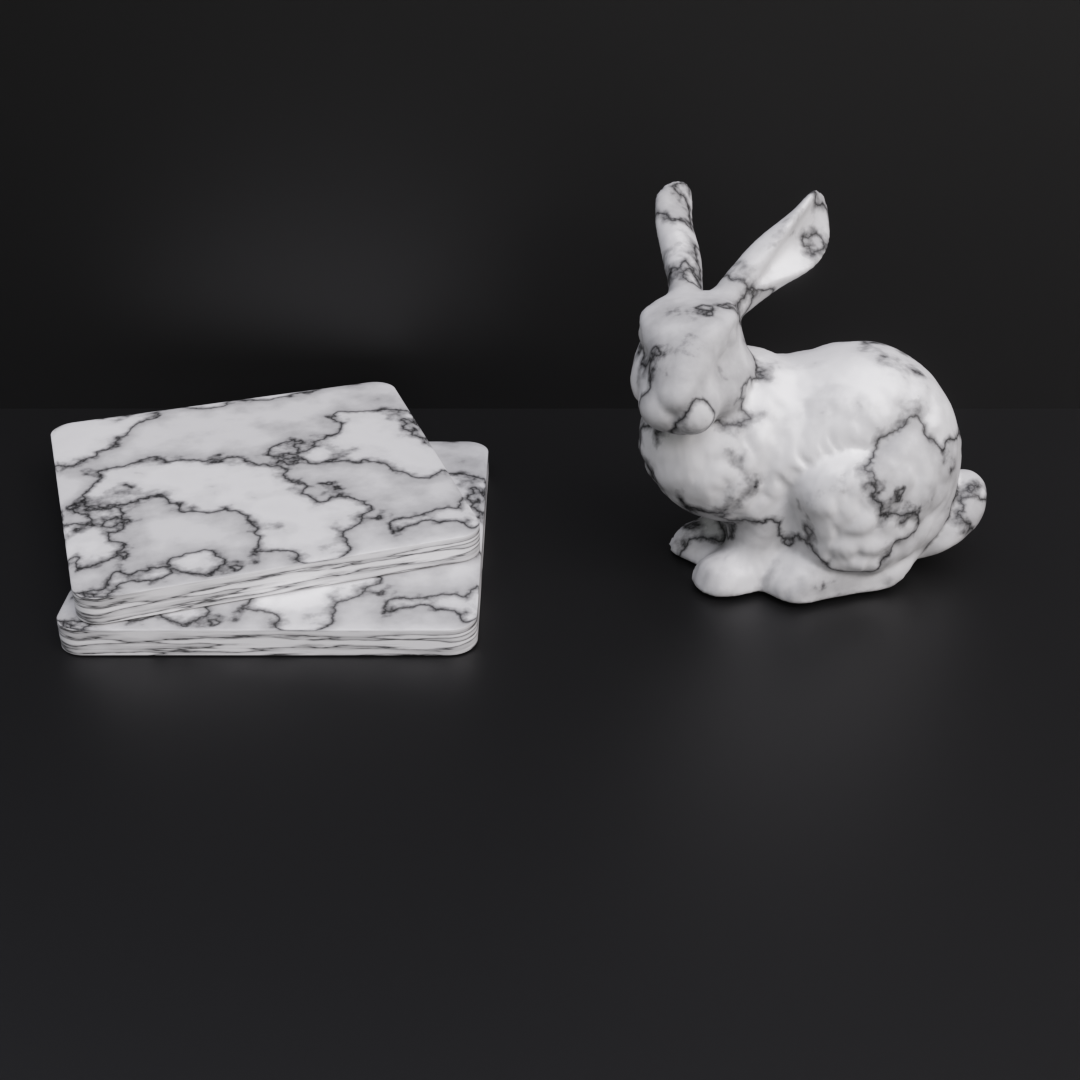
\includegraphics[width=0.7\linewidth]{./renders/marble_1024.png}
    \caption{Marble texture render with Stanford bunny and tiles, black background. Rendered until convergence in a 1080x1080 frame. See \texttt{./project/renders/marble\_1024.png} for clearer version.}
    \label{fig:marble}
\end{figure}

\subsection{Wood}
For the wood texture there is a bit more attention to detail for the natural structure of the material. Here the special object is a set of wooden planks. The result of this render can be seen in \autopageref{fig:wood}. 
Here the wood texture actually looks believable, apart from the fact that they may be cut a little too clean i.e. lacking some displacement. The wood rings follow a natural-looking pattern, which also works well on the flat surface of the plank.
What could be lacking is some knots in the wood, which often occur where branches have been on the tree, but since these are not always visible on processed wood it is a forgivable omission.
Looking at the reference bunny, it is a bit more clear that the texture is rendered as a wood worker probably wouldn't cut the would as a whole piece from the middle of the trunk like the texture does.
However, it was a bit out of the scope of this project and my abilities to simulate real wood carving. In general this render proposes a believable wood texture, in which the main ask is a computed displacement for the texture, which brings us to the last texture.

\begin{figure}[ht]
    \centering
    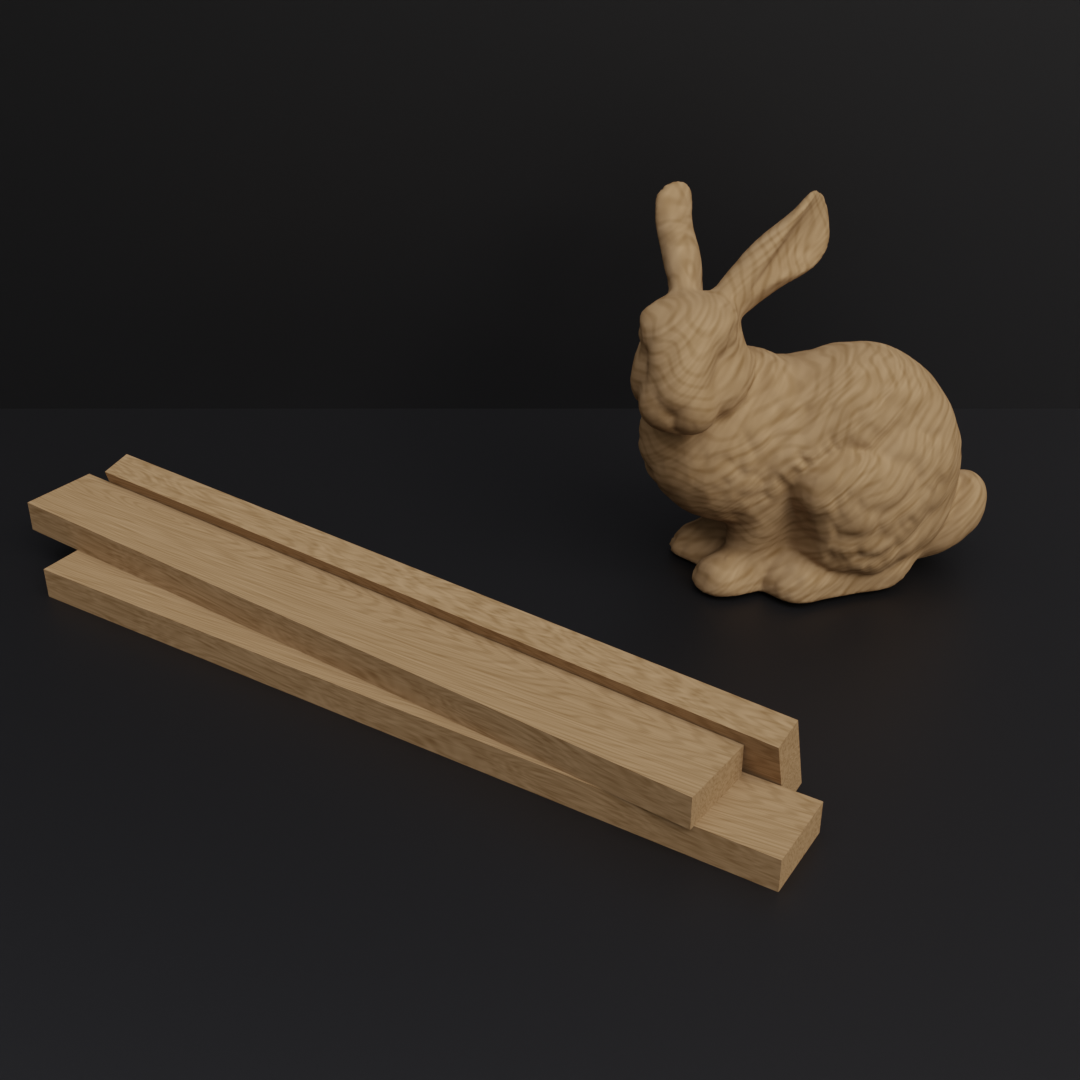
\includegraphics[width=0.7\linewidth]{./renders/wood_1024.png}
    \caption{Wood texture render with Stanford bunny and wooden planks, black background. Rendered until convergence in a 1080x1080 frame. See \texttt{./project/renders/wood\_1024.png} for clearer version.}
    \label{fig:wood}
\end{figure}

\subsection{Rocky Lava}
It an important note for this texture that it was originally developed on a Blender icosphere object (with 6 subdivisions), i.e. an object with a large number if small triangles that makes a sphere-like object.
This is important for how the displacement in the texture is created. For that reason the special object for this texture is an icosphere. The results for this render can be seen in \autoref{fig:lava}.
The first thing one might notice is, that the Stanford bunny now looks like a miserable burnt pigeon. That is due to the displacement and how it works on trimesh objects.
While the icosphere is made of standard small triangles with identical properties, the trimesh object is not. Here the triangles are of different sizes and are shaped quite differently. 
This does not play well with the displacement logic. On a more smooth trimesh object, like the one shown in \autoref{fig:lava_elephant} it works a lot better. 

Apart from the misshaped bunny, there icosphere turned out quite well. The glow resembles what one (who admittedly has never seen real lava) might expect, with the colors somewhat matching those, which are created by high temperatures of lava.
The rocky parts are sticking out with expected sharp edges, and the mixing of textures and displacements looks random and natural. 
Of course, lava usually doesn't clump into a ball like it is in the image, but mapped to a proper "river"-like object this could be believable.

\begin{figure}[ht]
    \centering
    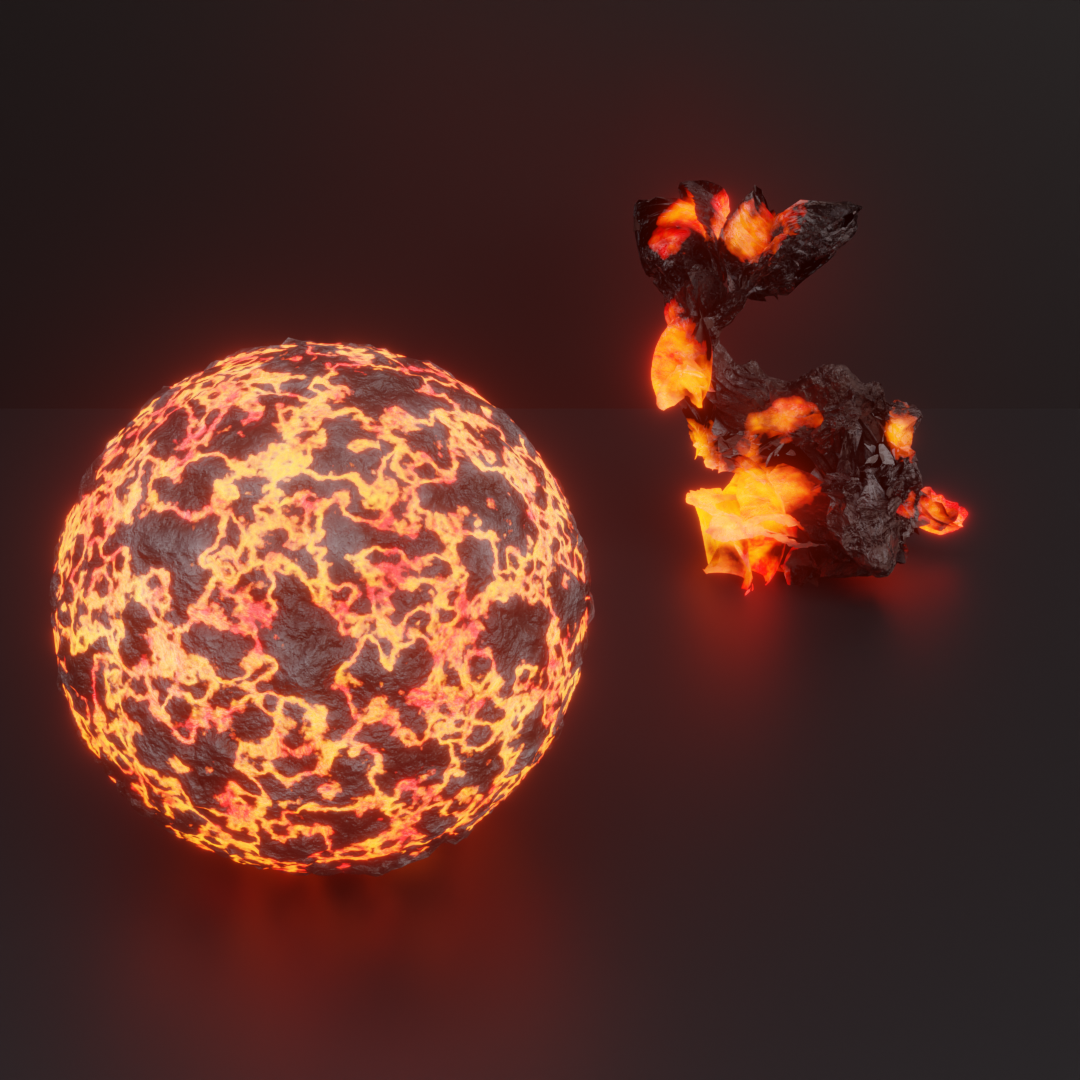
\includegraphics[width=0.7\linewidth]{./renders/lava_sphere_1024.png}
    \caption{Rocky lava texture render with Stanford bunny and lava ball, black background. Rendered until convergence in a 1080x1080 frame. See \texttt{./project/renders/lava\_sphere\_1024.png} for clearer version.}
    \label{fig:lava}
\end{figure}

\section{Discussion}


\newpage
\bibliography{sample}

\newpage
\appendix
\section{- Extra Rocky Lava texture renderings}
\begin{figure}[ht]
    \centering
    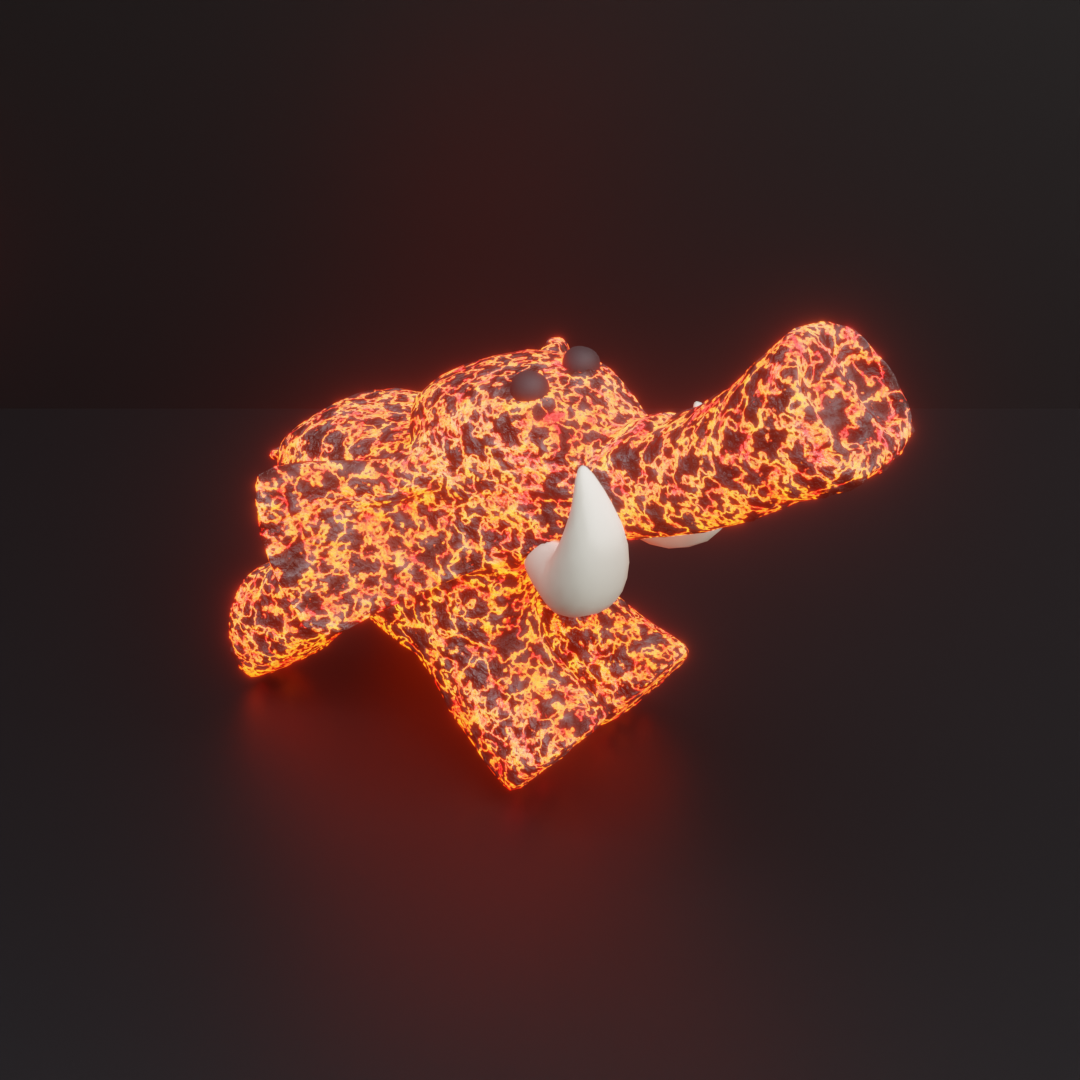
\includegraphics[width=0.85\linewidth]{./renders/lava_elephant_1024.png}
    \caption{Rocky lava texture render with Elephant and black background. Rendered until convergence in a 1080x1080 frame. See \texttt{./project/renders/lava\_elephant\_1024.png} for clearer version.}
    \label{fig:lava_elephant}
\end{figure}

\end{document}